\section{Background and Motivation}
\label{motivations}

In this section we present the background on state of the art
techniques that have been developed to handle data non-determinism
arising from complex data structures. We present an overview of lazy
initialization and lazier\# initialization. We also present a brief
description of the two bounding strategies used in symbolic execution
in heap manipulating programs. Next we present a motivating examples
where current concrete initialization of the heap structures struggle
to scale to medium sized program due to non-determinism introduced in
the symbolic execution tree. We use this example to motivate the need
for a more truly symbolic and compact representation of the heap in a
manner similar to that of primitive types.

Generalized symbolic execution technique generates a concrete
representation of connected memory structures using only the implicit
information from the program itself.  In the original lazy
initialization algorithm, symbolic execution explores different heap
shapes by concretizing the heap at the first memory access (read) to
an un-initialized symbolic object. At this point, a non-deterministic
choice point of concreate heap locations is created that includes: (a)
null, (b) an access to a new instance of the object, and (c) aliases
to other type-compatible symbolic objects that have been concretized
along the same execution path~\cite{GSE:TACAS2003}.  The number of
choices explored in lazy initialization greatly increases the
non-determinism and often makes the exploration of the program state
space intractable.

%Various improvements have been proposed to reduce the amount of
%nondeterminism from lazy initialization. One such optimization,
%introduced in \cite{Kiasan06} , is called lazier\#
%initialization.
The Lazier\# algorithm is an improvement of the lazy initialization
and it pushes the non-deterministic choices further into the execution
tree. In the case of a memory access to an uninitialized reference
location, by default, no choice point is created. Instead, the read
returns a unique symbolic reference representing the contents of the
location. The reference may assume any one of three states:
uninitialized, non-null, or initialized. The reference is returned in
an uninitialized state, and only in a subsequent memory access is the
reference concretely initialized.

\begin{figure}
\begin{tabular}[c]{l}
\begin{lstlisting}
public class LinkedList {

/** assume the linked list is valid with no cycles **/
LLNode head;
Data data0, data1, data2, data3, data4;

private class Data { Integer val; }

private class LLNode {
  protected Data elem;
  protected LLNode next; }

public static boolean contains(LLNode root, Data val) {
  LLNode node = root;
  while (true) {
    if(node.val == val)  return true;
    if(node.next == null) return false;
    node = node.next;
}}

public void run() {
if(LinkedList.contains(head, data0) && LinkedList.contains(head,data1) &&
   LinkedList.contains(head, data2) && LinkedList.contains(head, data3) &&
   LinkedList.contains(head, data4)) return;
\end{lstlisting}
\end{tabular} 
\caption{Linked list}
\label{fig:example}
\end{figure}

\begin{figure}[htb]
\scalebox{0.45}
{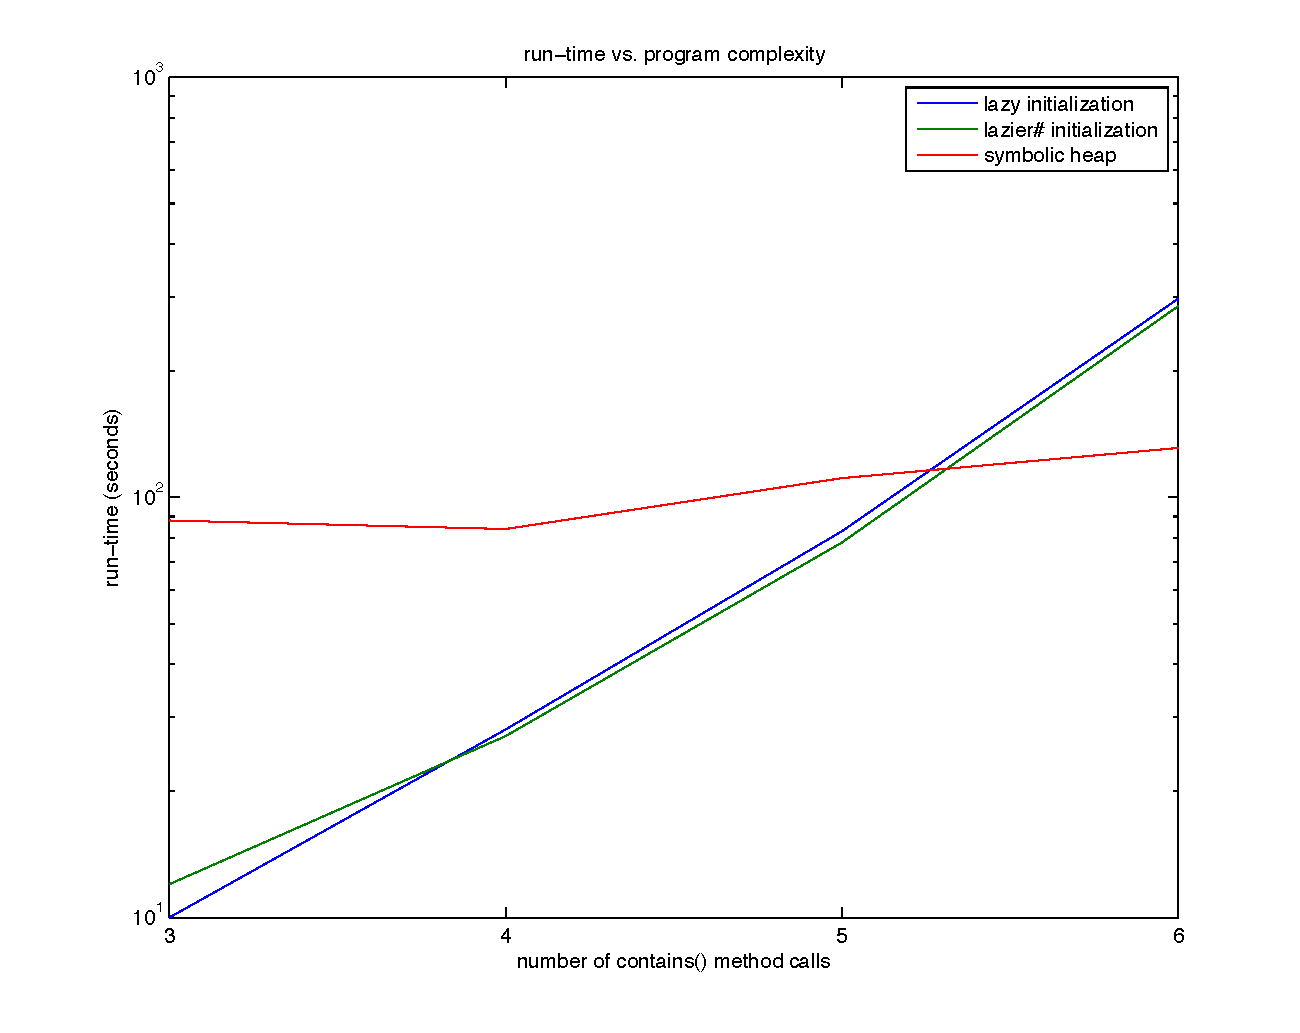
\includegraphics[width=563px]{../figs/time_vs_complexity.pdf}}
\caption{Time versus complexity for the linked list example}
\label{fig:tvc}
\end{figure}

